\chapter{Partialbråksuppdelning}
\paragraph*{Ex (6.2.16)} Beräkna $\int\frac{x^3+1}{12+7x+x^2}\, dx$.
\paragraph{Lösning}
Eftersom täljaren har en högre grad än nämnaren $(3>2)$ kan vi skriva om den rationella funktionen i integranden med hjälp av polynomdivision.
%infoga bild 1, longdivision
%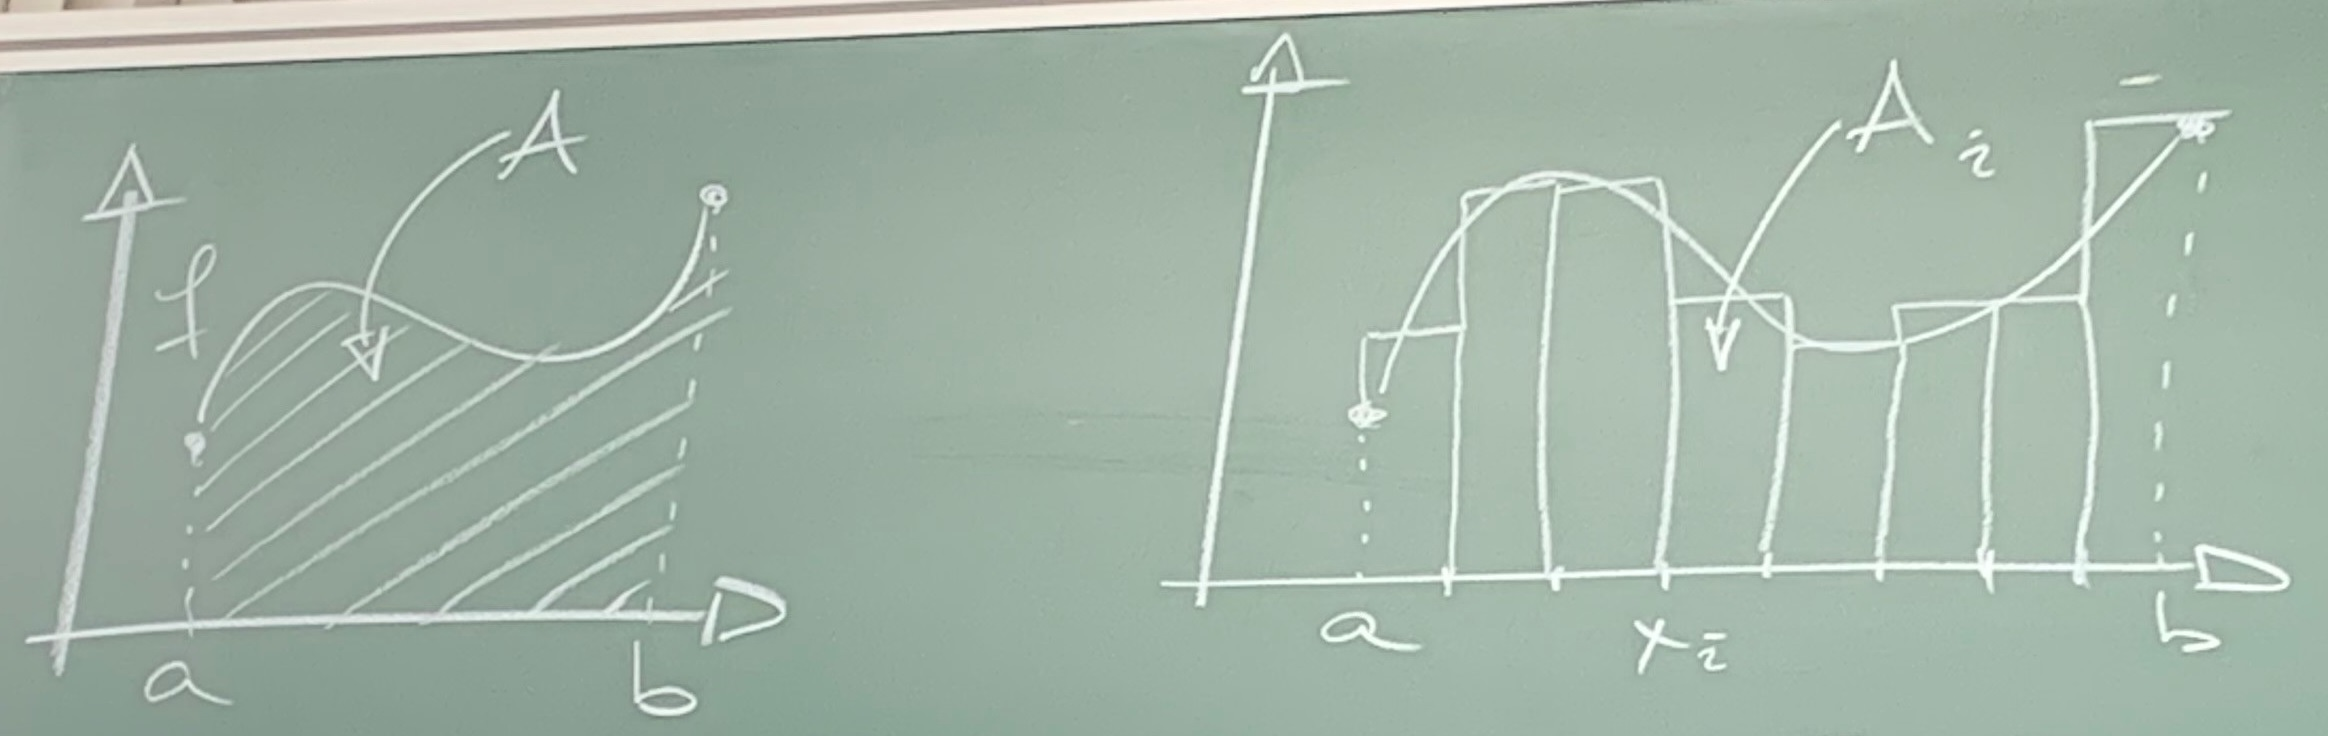
\includegraphics[]{lessons/lesson17/imgs/img01.jpg}
och alltså får vi att
\begin{equation*}
    \int\frac{x^3+1}{12+7x+x^2}\, dx=
    \int (x-7) + \int\frac{37x+85}{12+7x+x^2}\, dx=
    \frac{x^2}{2}-7x+\int\frac{37x+85}{12+7x+x^2}\, dx
\end{equation*}
Hur löser man den nya integralen som uppstår?
Polynomdivvision hjälper ej eftersom täljaren har lägre grad än nämnaren.
Faktorisera nämnaren genom att hitta dess nollställen!
\begin{equation*}
    12+7x+x^2=0\Rightarrow
    x^2+2\cdot \frac{7}{2}x+(\frac{7}{2})^2-(\frac{7}{2}^2)+12=0\Leftrightarrow
    (x+\frac{7}{2}^2)-\frac{49}{4}+12=0\Leftrightarrow
\end{equation*}
\begin{equation*}
    (x+\frac{7}{2}^2)=\frac{49}{4}-\frac{48}{4}=\frac{1}{4}\Leftrightarrow
    x=-\frac{7}{2}\pm\sqrt[]{\frac{1}{4}}=-\frac{7}{2}\pm\frac{1}{2}\Rightarrow
    \begin{matrix}
        x_1=-\frac{6}{2} \\
        x_2=-\frac{8}{2}=4
    \end{matrix}
\end{equation*}
Så $x^2+7x+12=(x+3)\cdot(x+4)$ så alltså
\begin{equation*}
    \int\frac{37x+85}{12+7x+x^2}\, dx=
    \int\frac{37x+85}{(x+3)\cdot(x+4)}\, dx=?
\end{equation*}
Prova följande \underline{ansats}:
\begin{equation*}
    \frac{37x+85}{(x+3)\cdot(x+4)}=
    \frac{A}{x+3}+\frac{B}{x+4},A,B\in\mathbb{R}
\end{equation*}
Finns talen $A$ och $B$ så att detta stämmer? Ja!
\begin{equation*}
    \frac{A}{x+3}+\frac{B}{x+4}=
    \frac{A(x+4)}{(x+3)(x+4)}+\frac{B(x+3)}{(x+3)(x+4)}=
    \frac{(A+B)x+(4A+3B)}{(x+3)(x+4)}
\end{equation*}
Alltså måste:
\begin{equation*}
    \left\lbrace
    \begin{matrix}
        A+B=37 \\
        4A+3B=85
    \end{matrix}
    \right.
    \Rightarrow...\Rightarrow
    \left\lbrace
    \begin{matrix}
        A=-26 \\
        B=63
    \end{matrix}
    \right.
\end{equation*}
$A$ och $B$ hittas dock enklast med den så kallade "handpåläggningsmetoden".
Börja med:
\begin{equation*}
    \frac{37x+85}{(x+3)(x+4)}=\frac{A}{x+3}+\frac{B}{x+4}
\end{equation*}
Multiplicera sedan med en nämnare:
\begin{equation*}
    \frac{37x+85}{(x+3)(x+4)}\cdot(x+3)=
    \frac{A(x+3)}{(x+3)}+\frac{B}{x+4}\cdot(x+3)=
    A+\frac{B}{x+4}\cdot(x+3)
\end{equation*}
När vi då sätter $x=-3$ försvinner $B$ och vi får värdet på $A$.
Gör likadant för andra värden.

Så
\begin{equation*}
    \int\frac{37x+85}{(x+3)(x+4)}\, dx=
    \int\frac{(-26)}{x+3}+\frac{63}{x+4}\, dx=
    63\int\frac{1}{x+4}\, dx -26\int\frac{1}{x+3}\, dx=
\end{equation*}
\begin{equation*}
    \{\int\frac{1}{x}\, dx=ln(|x|)+C\}=
    63\ln(|x+4|)-26\ln(|x+3|)+C,C\in\mathbb{R}
\end{equation*}
och vi har då alltså till slut fått:
\begin{equation*}
    \int\frac{x^3+1}{12+7x+x^2}\, dx=
    \int x-7+\frac{37x+85}{12+7x+x^2}\, dx=
    \frac{x^2}{2}-7x+63\ln(|x+4|)-26\ln(|x+3|)+C,C\in\mathbb{R}
\end{equation*}
Denna metod för att lösa integraler av typen $\int\frac{P(x)}{Q(x)}\, dx$ där $P$ och $Q$ är polynom kallas för \underline{partialbråksuppdelning}.
(Oftast underförstått att graden av $P$ är lägre än graden av $Q$).

\section{Sammanfattande om partialbråksuppdelning}
Om graden av $P$ är lägre än graden av $Q$ och $Q$ kan faktoriseras som \\
$Q(x)=(x-x_1)\cdot ... \cdot(x-x_n)$ så funkar ansatsen:
\begin{equation*}
    \frac{P(x)}{Q(x)}=\frac{A_1}{x-x_1}+\frac{A_2}{x-x_2}+...+\frac{A_n}{x-x_n}, A_1,A_2,...,A_n\in\mathbb{R}
\end{equation*}
förutsatt att alla nollställen $x_1,x_2,...,x_n$ är unika.\\
Talen $A_1,A_2,...A_n$ kan beräknas genom handpåläggning, dvs.
\begin{equation*}
    A_i=\lim_{x\to x_i}(x-x_i)\frac{P(x)}{Q(x)}
\end{equation*}
för alla $i=1,2,...,n$.\\
Vad händer om några av faktorerna $(x-x_1),(x-x_2),...,(x-x_n)$ är samma?
Till exempel om $Q(x)=(x-1)(x-2)^2(x-3)^3$?
Då gäller ansatsen:
\begin{equation*}
    \frac{P(x)}{Q(x)}=\frac{A_1}{(x-x_1)}+\frac{A_2}{(x-x_2)}+\frac{A_3}{(x-x_2)^2}+\frac{A_4}{(x-x_4)}+\frac{A_5}{(x-x_3)^2}+\frac{A_6}{(x-x_3)^3}
\end{equation*}
I dessa fall funkar ej handpåläggning och man måste lösa det linjära ekvationssystem enligt tidigare exempel.\\
Om $Q$ inte faktoriserar till linjära termer?
Till exempel $Q(x)=(x-1)(x^2+1)$?
Då gäller
\begin{equation*}
    \frac{P(x)}{Q(x)}=\frac{A}{x-1}+\frac{Bx+C}{x^2+1}
\end{equation*}
Osv... Läs vidare i kap 6.3.

\chapter{Inverssubstitutioner}
Variant av variabelsubstitution där man istället för att ersätta en funktion av $x$ med en ny variabel $u$ ersätter $x$ men en ny funktion av $u$.
Alltså:
\begin{equation*}
    \left\lbrace
    \begin{matrix}
        u=f(x) \\
        du=f^\prime(x)\, dx
    \end{matrix}
    \right. \underrightarrow{invers substitution}
    \begin{matrix}
        x=g(u) \\
        dx=g^\prime(u)\, du
    \end{matrix}
\end{equation*}
Gör integralen till synes svårare, men underlättar i vissa speciella situationer.

\paragraph{Ex (6.3.5)} Beräkna $\int\frac{dx}{x^2\sqrt{9-x^2}}$.
\subparagraph{Lösning} För integrander som innehåller
$\sqrt{a^2-x^2}, (a>0)$ brukar Inverssubstitutionen $x=a\sin(u)$ vara bra.
\begin{equation*}
    \int\frac{dx}{x^2\sqrt{9-x^2}}=
    \left\lbrace
    \begin{matrix}
        x=3\sin(u) \\
        dx=3\cos(u)
    \end{matrix}
    \right.=
    \int\frac{3\cos(u)\, du}{9\sin^2(u)\sqrt{9-9\sin^2(u)}}=
\end{equation*}
\begin{equation*}
    \int\frac{\cos(u)}{9\sin^2(u)\sqrt{1-sin^2(u)}}\, du=
    \{1-\sin^2(u)=\cos^2(u)\}=
\end{equation*}
\begin{equation*}
    \int\frac{\cos(u)}{9\sin^2(u)\sqrt(cos^2(u))}\, du=
\end{equation*}
\begin{equation*}
    \{\frac{1}{\sqrt{9-x^2}}\Rightarrow
    -3<x<3\Rightarrow -1<sin(u)<1\Rightarrow
    -\frac{\pi}{2}<u<\frac{\pi}{2}\Rightarrow
    cos(u)>0\}=
\end{equation*}
\begin{equation*}
    \int\frac{\cos(u)}{9\sin^2(u)\cdot\cos(u)}\, du=
    \int\frac{1}{9sin^2(u)}\, du=
    \frac{1}{9}\int\frac{1}{\frac{\sin^2(u)}{\cos^2(u)}}\cdot\frac{1}{cos^2(u)}\, du=
\end{equation*}
\begin{equation*}
    \frac{1}{9}\int\frac{1}{tan^2(u)}\cdot\frac{1}{\cos^2(u)}\, du=
    \left\lbrace
    \begin{matrix}
        tan(u)=w \\
        \frac{1}{\cos^2(u)}\, du=dw
    \end{matrix}
    \right.=
    \frac{1}{9}\int\frac{1}{w^2}\, dw=
    \frac{1}{9}(-\frac{1}{w})+C=
\end{equation*}
\begin{equation*}
    -\frac{1}{9}\cdot\frac{1}{\tan(u)}+C, C\in\mathbb{R}
\end{equation*}
Hur uttrycks detta i termer av $x$?
Använd rätvinkliga trianglar!
Vi satte $x=3\sin(u)$, dvs. $sin(u)=\frac{x}{3}$.
Betrakta följande triangel:\\
%infoga bild 2
%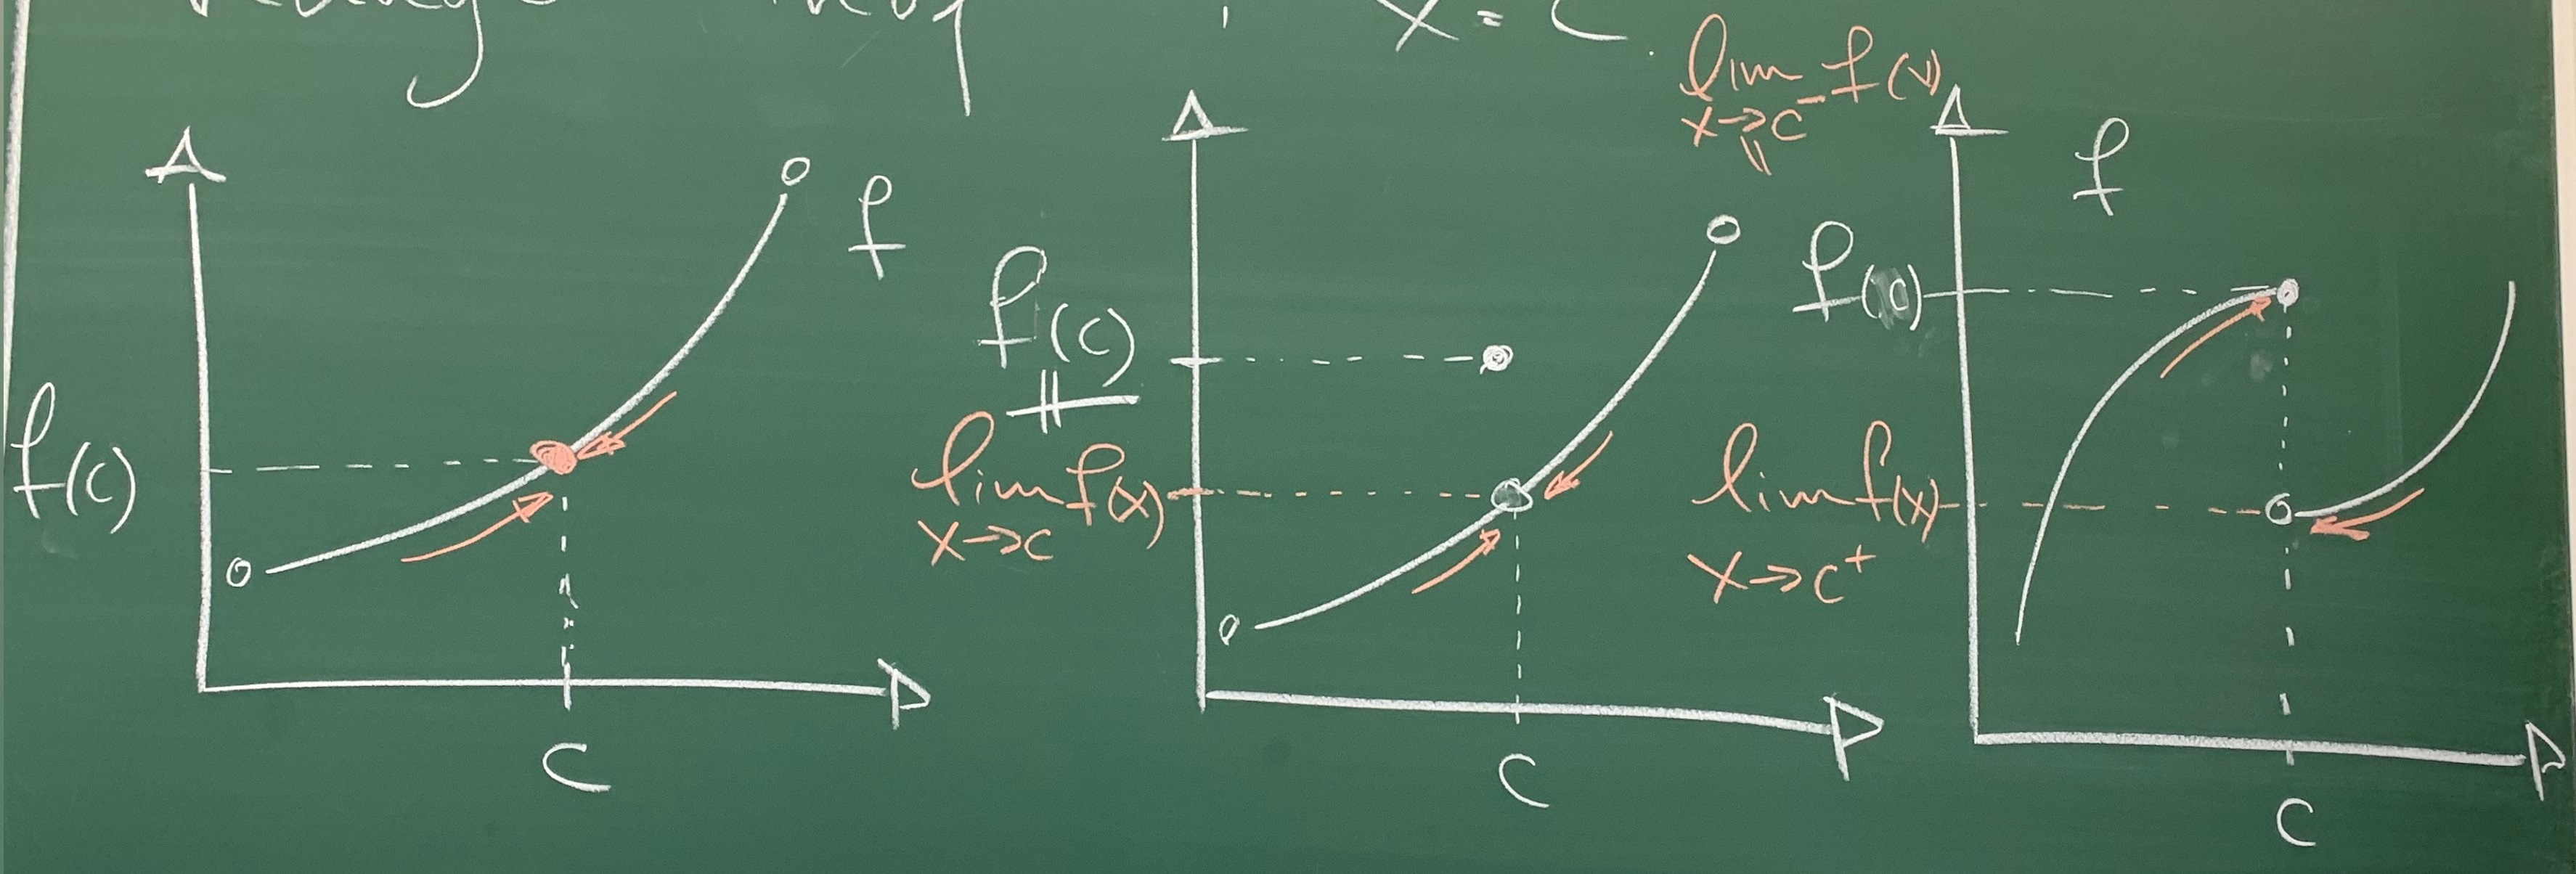
\includegraphics[]{lessons/lesson17/imgs/img02.jpg}
Här är uppenbarligen $\sin(u)=\frac{x}{3}$ dvs. $x=3\sin(u)$ (inv. subst.),
men även $\tan(u)=\frac{x}{\sqrt{9-x^2}}$.
Använd detta!
\begin{equation*}
    \Rightarrow\int\frac{dx}{x^2\sqrt{9-x^2}}=...=
    -\frac{1}{9}\cdot\frac{1}{\tan(u)}+C=
    -\frac{1}{9}\cdot\frac{\sqrt(9-x^2)}{x}+C,C\in\mathbb{R} \Box
\end{equation*}